\documentclass[conference]{IEEEtran}
\usepackage[T1]{fontenc}
\usepackage{amsmath}
\usepackage{graphicx}

\title{Capacitor Charging and a Power On Reset
for an Active Low Microcontroller}

\author{
\IEEEauthorblockN{Ali Hussain}
\IEEEauthorblockA{
Department of Computer Engineering Technology\\
Vanier College
}
}

\begin{document}
\maketitle

\begin{abstract}
This report looks at how a capacitor charges in an RC circuit and how
the same idea can be used for a simple power-on-reset circuit. The
charging curve is compared for different resistor values, and the reset
release time is calculated for an active-low microcontroller reset pin.
\end{abstract}

\section{Introduction}

When a capacitor $C$ charges through a resistor $R$ from a constant
supply voltage $V_0$, the capacitor voltage is

\begin{equation}
V(t)=V_0\left(1-e^{-t/RC}\right).
\end{equation}

The product $RC$ is called the time constant,

\begin{equation}
\tau=RC.
\end{equation}

At one time constant,

\begin{equation}
V(\tau)=V_0\left(1-e^{-1}\right)
\approx 0.632V_0.
\end{equation}

For a supply voltage of $5.0$ V,

\begin{equation}
V(\tau)\approx 0.632(5.0)
\approx 3.16\text{ V}.
\end{equation}

Figure~\ref{fig:rc} compares the charging curve for different resistor
values while keeping the capacitor value constant.

\begin{figure}[t]
\centering
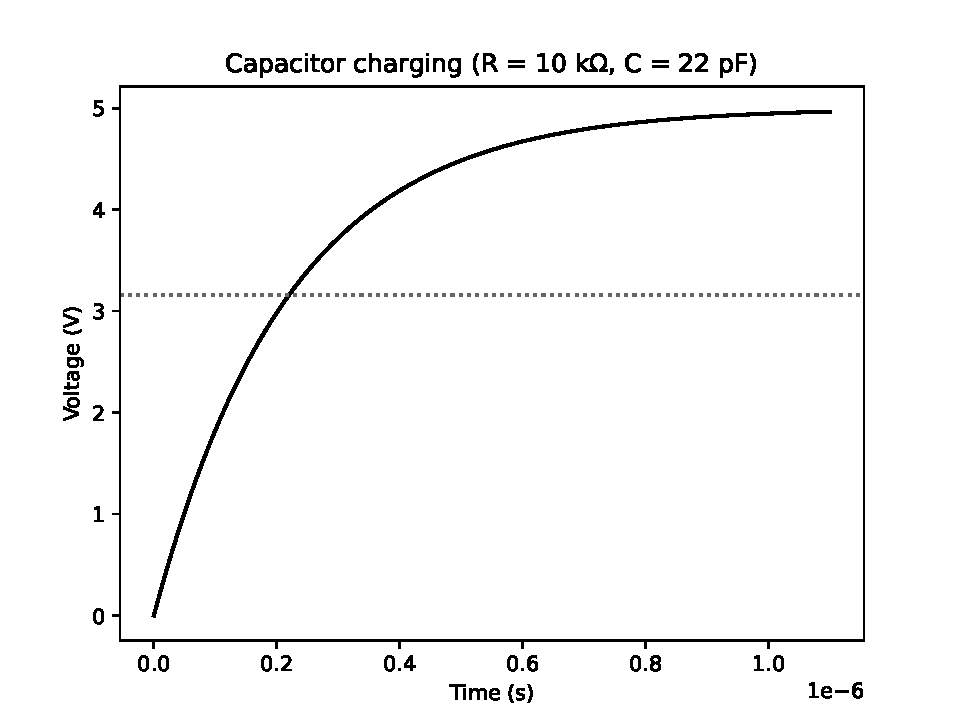
\includegraphics[width=\columnwidth]
{../figures/generated/rc_charging.pdf}
\caption{Capacitor charging for different resistor values with
$C=22\,\text{pF}$.}
\label{fig:rc}
\end{figure}

\section{Power On Reset}

An RC circuit can also be used as a simple power-on-reset circuit for
a microcontroller with an active-low reset pin. When power is first
turned on, the capacitor starts discharged, so the reset node is low.
As the capacitor charges through the resistor, the voltage at the reset
pin increases.

The reset is released when the voltage reaches the input-high threshold
$V_{IH}$.

\begin{figure}[t]
\centering
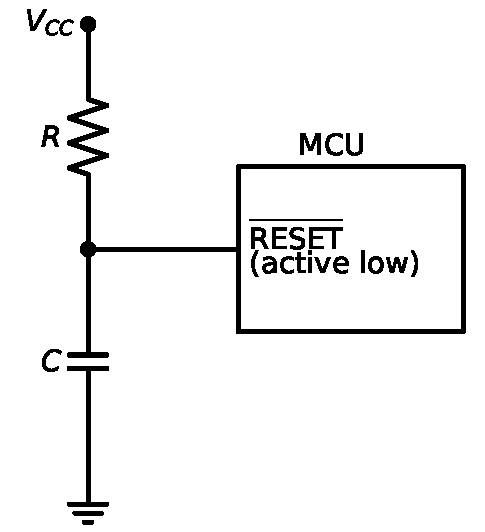
\includegraphics[width=\columnwidth]
{../figures/drawn/por_circuit.pdf}
\caption{RC power-on-reset circuit connected to an active-low reset pin.}
\label{fig:por}
\end{figure}

Starting from the charging equation and setting the capacitor voltage
equal to $V_{IH}$,

\begin{equation}
V_{IH}=V_0\left(1-e^{-t_{\text{release}}/RC}\right).
\end{equation}

Rearranging gives

\begin{equation}
t_{\text{release}}
=
-RC\ln\left(1-\frac{V_{IH}}{V_0}\right).
\end{equation}

If the required release time is known, the equation can also be solved
for $R$:

\begin{equation}
R=
\frac{-t_{\text{release}}}
{C\ln\left(1-\frac{V_{IH}}{V_0}\right)}.
\end{equation}

For this example,

\[
V_{IH}=0.7V_0,
\]

\[
V_0=5.0\text{ V},
\]

\[
t_{\text{release}}=10\text{ ms},
\]

and

\[
C=100\text{ nF}.
\]

First,

\begin{equation}
\ln(1-0.7)=\ln(0.3)\approx -1.204.
\end{equation}

Then,

\begin{equation}
R=
\frac{-(10\times10^{-3})}
{(100\times10^{-9})(-1.204)}
\approx 83\,\text{k}\Omega.
\end{equation}

Therefore, using an $83\,\text{k}\Omega$ resistor and a $100$ nF
capacitor gives a reset delay of about 10 ms.

\end{document}
